\documentclass{ctexart}
\usepackage{geometry}
\geometry{left=2.5cm, right=2.5cm, top=3.5cm, bottom=3.5cm}
\usepackage{amssymb}
\usepackage{bm}
\usepackage{amstext}
\usepackage{graphicx}
\usepackage{cancel}
\usepackage{algorithm}
\usepackage{algorithmic} 

\begin{document}
	\title{关于生成式对抗网络的综述}
	\author{石博天 (3120160454)}
	\date{\today}
	
	\maketitle
	\begin{section}{生成式对抗网络}
		2014年,由Goodfellow等人发表了一篇文章\cite{goodfellow2014generative},讨论了一种名为“生成式神经网络(Generative Adversarial Nets)的结构。
		生成式对抗网络是一类解决问题的框架,并且依托于这个思路,能够定义出多种不同的结构来,本文则是定义了一种特殊的情况:生成模型通过输入一段噪声来生成数据。作者将这个特殊情况称为对抗网络。
		
		生成对抗网络主要包含生成器(Generator)和判别器(Discriminator)两个部分。 生成器输入一段由$p_z$随机采样得到的噪声,输出为生成的样本。 判别器需要能判别输入的样本是由数据分布$p_{data}$生成的,还是由生成器$p_g$生成的。本文作者直接使用多层感知其(MLP)作为生成器和判别器。并使用了dropout等来提升效果。
		
		网络的目的之一,就是通过数据$x$学习到生成器的概率分布$p_g$。模型首先定义了一个输入噪声的随机变量$p_z(z)$,然后将由这个分布采样出来的噪声$z$经过映射$G(z;\theta_g)$映射到数据空间。也就是说,如果这个由参数$\theta_g$控制的$G$足够强大、参数选择的足够好,则将噪声映射到的那个数据空间,应该跟训练数据的数据空间相一致。这就说明,通过训练,我们可以用$G$将一组随机噪声mapping到一个“真实”的数据。这里“真实”加了引号,是因为这个真实指的不是训练数据中的某个真实样例,而是由生成真实数据的生成模型$p_g$所生成的其他数据。可见,这个生成模型其实能够生成“新东西”,也就是“符合数据的概率分布、但与已知训练数据都不相同”的真实内容。
		
		至此,我们就可以构建出一个生成模型。但仔细一想,现有的手段并不能满足我们“产生新知识”的要求:如果我们只有一个生成模型,那么训练的目标函数是什么?是已有的数据?
		
		如果训练目标是已有的数据,那这个问题就退化成了无监督的回归问题:让生成器$G$的输出尽可能与已有的样本相等。但是这种方法并不能训练处新知识,而只是让生成器“记住更多训练数据”。
		
		所以,作者很巧妙地增加了另一个模块:判别器$D$。
		
		判别器的作用就是判别刚刚生成的数据是“真实的样本”?还是“由生成器生成出来的样本?”如此一来,这个整体模型就变成了两方博弈的过程:生成器学习如何去伪造尽可能逼真的数据,判别器学习如何鉴别出那些是生成的数据、哪些是真实的数据。
		
		也就是说,这个模型由两个部分共同组成。我们可以定义如下的优化目标函数:
		
		\begin{equation}
		\mathop{\min}_{G}\mathop{\max}_{D}V(D,G)=\mathbb{E}_{\bm{x}\sim p_{\text{data}}}\left[\log D(\bm{x})\right]+\mathbb{E}_{\bm{z}\sim p_z(\bm{z})}\left[\log(1-D(G(\bm{z})))\right].
		\end{equation}
		
		这个目标函数的含义,就是找到一个能让这个函数最大化的$D$和最小化的$G$。因为这个函数越大,则说明$D$的判别能力越强。而这个函数越小,说明$G$的“伪装”能力越强(生成的样本越像真实样本)。
		
		听上去有些矛盾是不是?但实际上,这个最大化且最小化的模型,就像两个对手相互竞争,最终达到收敛。作者在文章中证明:这个训练过程总会收敛,而且收敛时,$p_g=p_{data}$,而优化函数则会收敛到$-\log4$
		
		在模型的训练过程中也有一些潜在的问题。
		
		首先是由于整个数据集比较大,在内层循环中利用整个数据集去优化$D$的过程是难以计算的,所以我们用迭代的方式:先训练$k$)次$D$,然后训练一次$G$。这样能够让$G$变化的缓慢一些,防止过拟合。
		
		还有一个问题就是,由于上面这个优化的目标函数不能对$G$的更新提供足够的梯度。并且在训练初期,$G$显然是一个非常差的模型,这个时候$D$有很高的可能性会鉴别出来$G$)生成的“伪”数据。因为这些数据与真实数据相比确实是非常的不同。而在这种情况下,$\log(1-D(G(\boldsymbol{z})))$饱和了。所以此时,我们不再最小化$\log(1-D(G(\boldsymbol{z}))$而是去训练$G$去最大化$\log(D(G(\boldsymbol{z})))$。这种训练方法会导致"The same fixed point of the dynamics of $G$ and $D$",但是能够在训练的早期提供比较大的梯度。
		
		让我们直观一些解释一下。我们本来需要优化的函数是同时最大最小化这个函数:
		
		\begin{equation}
			\mathop{\min}_{G}\mathop{\max}_{D}V(D,G)=\mathbb{E}_{\boldsymbol{x}\sim p_{\text{data}}}\left[\log D(\boldsymbol{x})\right]+\mathbb{E}_{\boldsymbol{z}\sim p_z(\boldsymbol{z})}\left[\log(1-D(G(\boldsymbol{z})))\right].
		\end{equation}
		
		但因为上面公式的第二项(有生成器的那部分)的形式会导致其很容易处于饱和状态(即梯度几乎是0的状态)。这时候对我们的训练时非常不利的!所以我们将这个训练过程拆成两步。第一步是按照上面的损失函数\emph{只}训练判别器。然后再换一个目标函数来训练生成器:
		
		\begin{equation}
			\mathop{\max}_{D}\mathbb{E}_{\boldsymbol{x}\sim p_{\text{data}}}\left[\log D(\boldsymbol{x})\right]+\mathbb{E}_{\boldsymbol{z}\sim p_z(\boldsymbol{z})}\left[\log(1-D(G(\boldsymbol{z})))\right]\\\\
			\mathop{\max}_{G}\mathbb{E}_{\boldsymbol{z}\sim p_{\text{z}}}\left[\log D(G(\boldsymbol{z}))\right]
		\end{equation}
		
		这两个部分交替进行训练,也就是本片论文中提到的“训练$k$次$D$、训练一次$G$”
		
		在文章的实验部分,作者使用了几个不同的数据集进行训练,结果如图\ref{fig:gan-example}所示。
		
		\begin{figure}
			\centering
			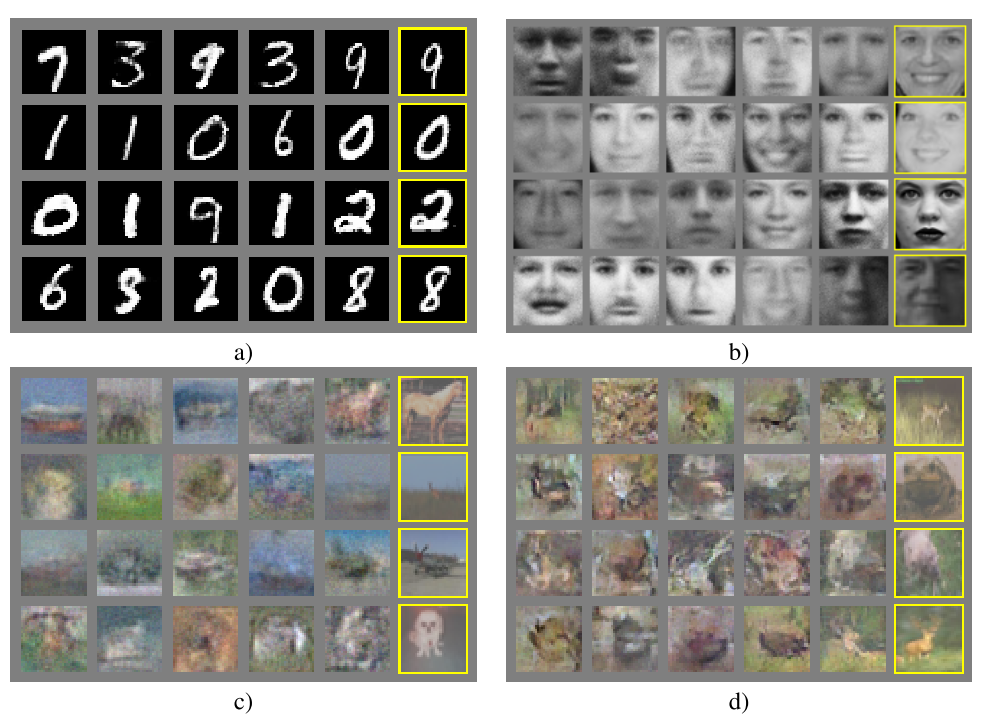
\includegraphics[width=30em]{figures/GAN-experiment-demo-pic.PNG}
			\caption{GAN示例}
			\label{fig:gan-example}
		\end{figure}
	
		图\ref{fig:gan-example}中的每一副图片都是由一个数据集生成。图片左边五列是生成的内容,最后一列是与第四列生成出内容最像的一个。从结果上能看出来:生成的模型与真实模型相似、但不完全一致。说明我们的目标达到了。
		
		作为一篇用来首次提出模型的文章,这个模型还很简单,所以文章的精华部分在于讨论这个模型的优缺点以及后续的可能的工作,相当于给后来人留下许多可以进行的工作。
		
		首先,文章自己承认,用这种方法其实并不能学习到一个明确的$p_g(\boldsymbol{x})$的表示,由于里面用了神经网络,所以最后只相当于学习到了一个黑盒子:以噪声为输入,以生成的结果为输出。除此之外,判别器的训练过程应该与生成器的训练过程保持同步。特别在判别器没有更新的情况下,绝对不能更新太多次生成器,否则可能会发生“Helvetica Scenario”现象,也就是不论$\boldsymbol{z}$是啥,都会得到同样的生成结果$\boldsymbol{x}$。
		
		而这个模型的好处在于不需要马尔科夫链,只需要用反向传导的算法获取梯度即可,并且在学习过程中也不需要推断过程。
		
		论文中列了个表格来讨论GAN与其他模型的优劣,详情如图\ref{fig:gan-comparison}
		\begin{figure}
			\centering
			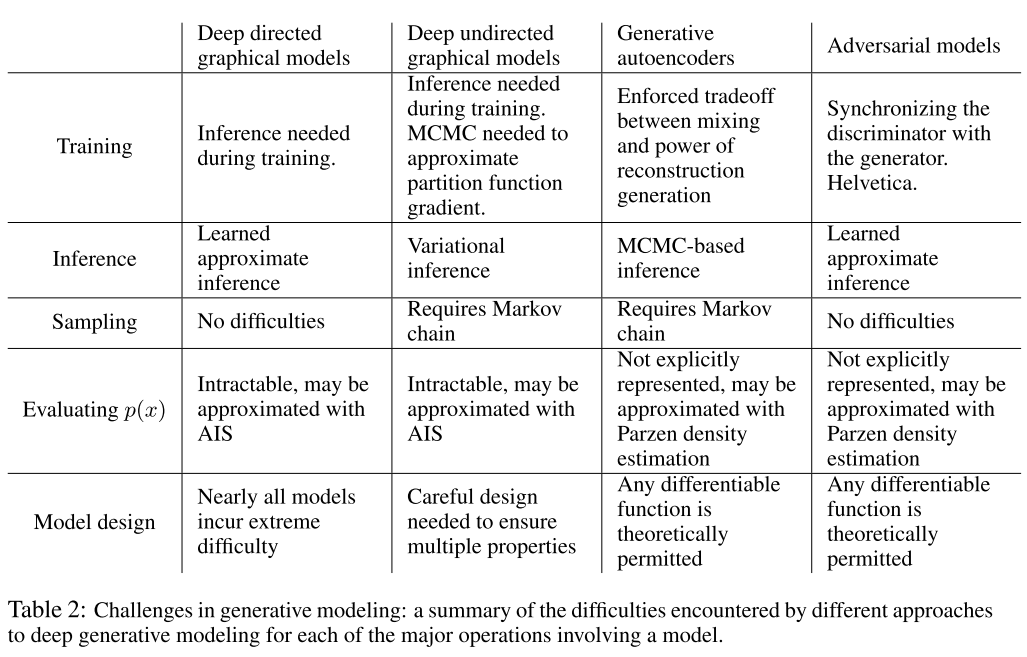
\includegraphics[width=40em]{document-figures/gan-comparison.png}
			\caption{GAN与其他模型的对比分析}
			\label{fig:gan-comparison}
		\end{figure}
	
		其中文翻译如图\ref{fig:gan-comparison-ch}
		
		\begin{figure}
			\centering
			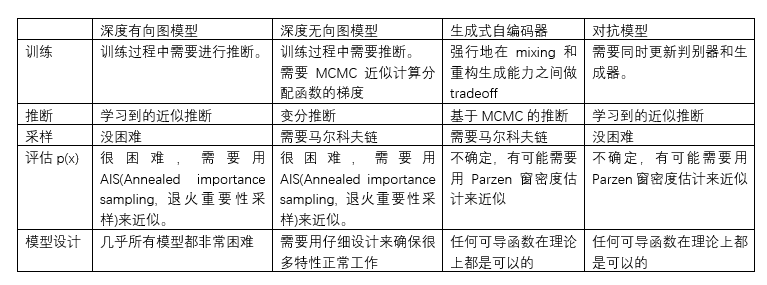
\includegraphics[width=40em]{document-figures/gan-comparison-ch.png}
			\caption{GAN与其他模型的对比分析}
			\label{fig:gan-comparison-ch}
		\end{figure}
	
		GAN的优点主要是“可计算”。对抗模型在统计特性上也有一些优势,比如说生成器并不是直接通过数据样本进行更新,而是通过判别器的梯度进行更新。这意味着算法并不是直接将输入数据拷贝到生成器的参数中(而是学习到了样本数据的一些特征)。另一个对抗网络的好处是它能够表现的非常“锐”,甚至是对退化分布也是如此。而基于马尔科夫链的方法需要这个分布有一些模糊才能够使得其能够融合多个模式。
		
		紧接着,作者提出了几点在未来可能会有价值的扩展:
		\begin{enumerate}
			\item 通过在$G$和$D$上增加一个输入$\boldsymbol{c}$,从而能够得到一个“条件生成模型”$p(\boldsymbol{x}|\boldsymbol{c})$。
			\item 通过训练一个辅助的网络来用$\boldsymbol{x}$预测$\boldsymbol{z}$,从而能学习到近似推断。
			\item 能近似地建模所有条件概率$p(\boldsymbol{x}_S|\boldsymbol{x}_{\cancel{S}})$。其中的$S$是通过训练一组条件概率模型得到的共享参数的下标(indices)的子集。
			\item 半监督学习:当只有有限的标注数据时,判别器或者推断网络中得到的特征能够提高分类性能。
			\item 提升效率:可以通过一些能更好地协调$G$与$D$的方法或者更好的对$z$进行采样的方法来提升效率。
		\end{enumerate}
	
		最后作者说了一句意味深长的话:\emph{This paper has demonstrated the viability of the adversarial modeling framework, suggesting that these research directions could prove useful.}
		
		也就是说,作者提出了一个adversarial modeling framework,在这个framework上还是有不少可以继续研究的东西的。
	\end{section}	

	\begin{section}{Conditional Generative Adversarial Networks\cite{mirza2014conditional}}
		在上一节中我曾经介绍过Generative Adversarial Nets这个模型。
		
		这个框架包括一个生成器(Generator, G)和一个判别器(Discriminator, D)两个部分。生成器输入一段随机产生的噪声,生成一张尽可能“逼真”的图片。而判别器则输入一张图片,输出判断这张图片是生成出来的还是真实的。
		
		原作者Goodfellow在最早提出的这篇文章的最后,介绍了几个这个模型可能改进的方向。其中一个就是“A \emph{conditional generative} model $p(x|c)$ can be obtained by adding $c$ as input to both $G$ and $D$”。
		
		确实,GAN的原始模型有很多可以改进的缺点,首当其中就是“模型不可控”。从上面对GAN的介绍能够看出,模型以一个随机噪声为输入。显然,我们很难对输出的结构进行控制。例如,使用纯粹的GAN,我们可以训练出一个生成器:输入随机噪声,产生一张写着0-9某一个数字的图片。然而,在现实应用中,我们往往想要生成“指定”的一张图片。
		
		最直观的想法就是在GAN上增加一个额外的输入。也就是说,以前我们的生成模型是$p_g(x)$,现在,我们的生成模型是在一个条件$c$的控制下产生:$p_g(x|c)$。而这个$c$就是我们用来控制模型的额外的输入。
		
		$c$可以是表示我们意图的一串编码,例如我们想要做0-9的手写数字生成,则$c$可以是一个10维的one-hot向量。则在训练过程中,我们将这些label加入到训练数据中,从而得到一个按照我们需求产生图片的生成器。
		
		这就是Conditional Generative Adversarial Nets最基本的想法。这里要注意的是,这个$c$不但附加在了生成器上,同时也附加在了判别器上,相当于给了判别器一个额外的信息:现在这个图片是以条件$c$生成的?还是以条件$c$控制下的真正的图片?
		
		下面,我们介绍一下模型的基本结构。
		
		对于GAN来说,我们训练的目标是:
		\begin{equation}
			\mathop{\min}_{G}\mathop{\max}_{D}V(D,G)=\mathbb{E}_{\boldsymbol{x}\sim p_{\text{data}}}\left[\log D(\boldsymbol{x})\right]+\mathbb{E}_{\boldsymbol{z}\sim p_z(\boldsymbol{z})}\left[\log(1-D(G(\boldsymbol{z})))\right].
		\end{equation}
		
		而对于Conditional的GAN来说,训练目标只需要变成:
		
		\begin{equation}
			\mathop{\min}_{G}\mathop{\max}_{D}V(D,G)=\mathbb{E}_{\boldsymbol{x}\sim p_{\text{data}}}\left[\log D(\boldsymbol{x}|\boldsymbol{y})\right]+\mathbb{E}_{\boldsymbol{z}\sim p_z(\boldsymbol{z})}\left[\log(1-D(G(\boldsymbol{z}|\boldsymbol{y})|\boldsymbol{y}))\right].
		\end{equation}
		
		其实这个改动形象一些表示就是将原来只接受一个输入$z$的生成器变成接受两个输入($z$和$y$),将原来只接受一个输入$x$的判别器变成接受两个输入($x$和$y$)。再具体一些,如图\ref{fig:cgan-ori-struct},图右边绿色的部分就是条件,记为$y$。
		
		\begin{figure}
			\centering
			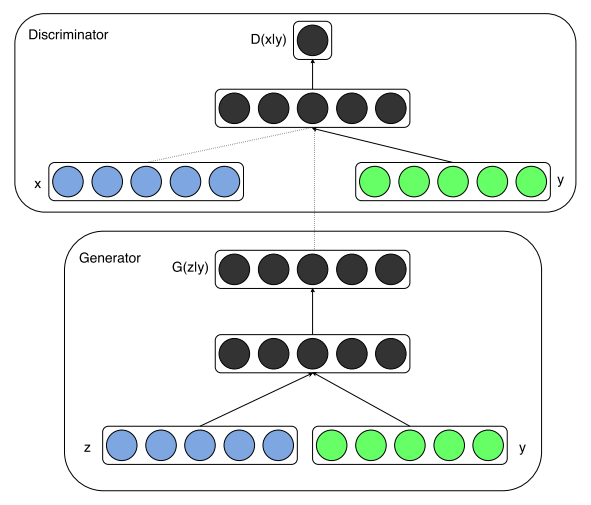
\includegraphics[width=25em]{figures/CGAN-origin-structure.png}
			\caption{Conditional Adversarial Nets}
			\label{fig:cgan-ori-struct}
		\end{figure}
	
		
		这个模型的思想非常简单,基本上一句话就讲明白了。紧接着就是实验部分了。
		
		实验分成了两种,一种是单模态,一种是多模态。
		
		单模态的试验以MNIST为数据集,控制输入$y$是label的one-hot表示。效果如图\ref{fig:cgan-exp-mnist}
		
		\begin{figure}
			\centering
			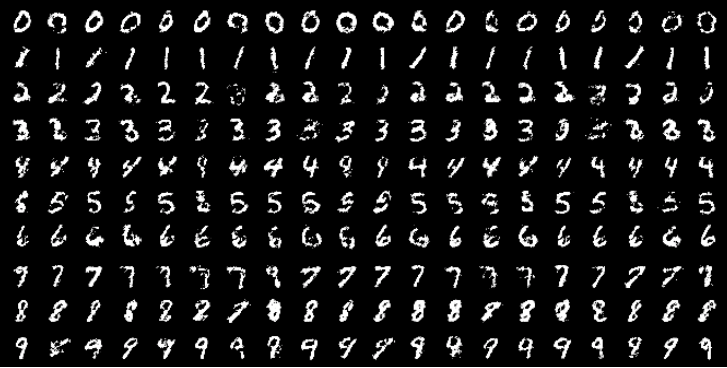
\includegraphics[width=25em]{figures/CGAN-experiment-mnist.png}
			\caption{根据MNIST数据集生成的数字。每一行是以一个label作为控制条件生成的}
			\label{fig:cgan-exp-mnist}
		\end{figure}
	
		多模态的实验比较复杂,作者做了一个图像自动标注。在这个Conditional GAN的框架下,模型有好多个部分。首先在完整的ImageNet数据集(21,000个label)上训练了一个卷积模型作为特征提取器。对于词语表达(原文中是world representation,个人认为是笔误,应该是word representation),作者使用YFCC100M数据集中的user-tags, titles和descriptions,利用skip-gram训练了一个200维的词向量。训练中忽略了词频小于200的词,最终词典大小是247465。
		
		在实验过程中,固定了这个卷积模型和词向量。生成器的输入$z$为噪声,输入$y$为经过卷积网络提取后得到的图片的特征(文中称是一个经卷积展开全连接隐层产生的4096维的向量)。判别器输入$x$为一个词向量,判别器的功能是判断这个词向量是否是对图片的正确标注。
		
		实验效果如图\ref{fig:cgan-exp-mul-mod}
		
		\begin{figure}
			\centering
			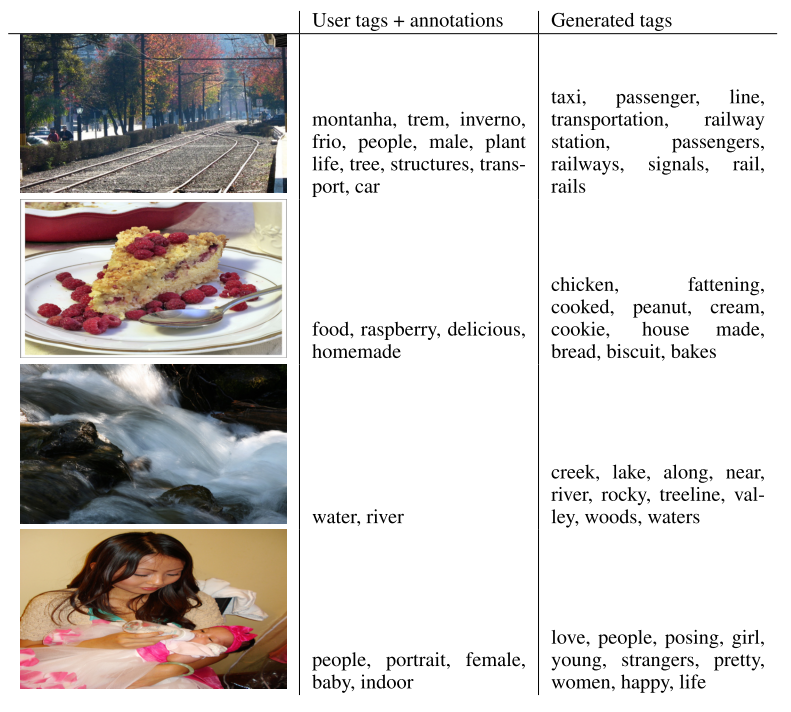
\includegraphics[width=25em]{figures/CGAN-experiment-multi-modal.png}
			\caption{多模态数据实验结果}
			\label{fig:cgan-exp-mul-mod}
		\end{figure}
		
		从实验结果来看,生成的标签还是很不错的。
		
	\end{section}


	\begin{section}{Deep Convolutional Generative Adversarial Networks}
		第一节中我们介绍过Generative Adversarial Nets这个模型。原作者Goodfellow在那篇文章\cite{goodfellow2014generative}中提出了一个基本的框架:生成器以一个随机采样的噪声向量作为输入,并输出一张图片。判别器用来判断这张图片是真实世界中的图片,还是由生成器产生的。在这个对抗(Adversarial)训练的过程中,生成器和判别器进行零和博弈并最终收敛。
		
		GAN这个框架有很多优点:收敛、不依赖马尔科夫链、只需要用BP算法计算梯度等。然而这个方法还有很多问题。
		
		首先,这种方法并不能学习到真正的数据分布$p_g(x)$。由于其中的生成器和判别器使用了神经网络,所以训练出来的生成模型更像一个黑盒子:给定输入,产生输出。而其中内部机制并不明晰。
		
		除此之外,训练过程并不稳定:训练器的训练过程应该与生成器的训练过程保持同步。特别在判别器没有更新的情况下,绝对不能更新太多次生成器,否则可能会发生“Helvetica Scenario”现象,也就是不论输入的随机采样的噪声向量$z$是啥,都会得到同样的生成结果$x$。
		
		本篇博客介绍的文章(Unsupervised Representation Learning with Deep Convolutional Generative Adversarial Networks\cite{radford2015unsupervised})就是在GAN的基础之上,引入了一系列约束(constraints),结合CNN(Convolutional Neural Nets)在一定程度上解决了这个问题。并且在后面附带了大量的实验来证实他们提出的这个模型的强大。
		
		首先,本篇论文的作者也认为GAN在训练中非常不稳定:
		> GANs have been known to be unstable to train. Often resulting in generators that produce nonsensical outputs.
		
		所以这篇文章在增加训练稳定性、提高特征学习能力等方面做了不少工作:
		
		\begin{enumerate}
			\item 作者提出了深度卷积GAN (Deep Convolutional GANs, DCGAN),并且在这个架构上增加了一些约束,使得在大多数情况下能够稳定地训练
			\item 作者将训练好的判别器(Discriminator)用来进行图片分类的任务,结果发现效果要比其他无监督的算法要好(可能是由于这种方法判别器能更好地学习到知识的特征表达)。
   			\item 作者将模型学习到的filters可视化,发现一些filters学习到了如何去“画”一些特殊的对象(也就是说学习到的filter是合理的靠谱的)。
			\item 作者发现生成器具备了“向量运算”的神奇性质,类似于word embedding可以操纵向量,并且能够按照“语义”生成新内容。
		\end{enumerate}
	
		下面将会介绍一下DCGAN的内容。
		
		对于卷积神经网络部分,作者用上了几个最近被证实有效的对CNN架构的修改。
		
		\begin{enumerate}
			\item 把所有的pooling (例如maxpooling)等用"stride"替代。这能让网络学习到自己的空间上的降采样。作者将这个方法用在了生成器(使用stride上采样)和判别器上。
			\item 去掉了卷积特征之后的全连接层。改用global average pooling,这虽然会影响收敛速度但是能增加模型的稳定性。
			\item 使用了Batch Normalization,这能够通过让输入到每一个节点的数据都保持0均值1方差,从而稳定训练,并且能够帮助训练更深层的模型。这个方法非常重要,它能够防止模型永远只能输出相同的样本,也就是上面提到的“Helvetica Scenario”现象。这个现象是GAN在实际使用中遇到的最大的问题。
		\end{enumerate}
	
		除此之外,作者在生成器中除了输出层以外,激活函数都是用ReLU,输出层激活函数使用Tanh。这能够让模型在训练中更快地达到饱和并且能对彩色样本有更好的效果。而且,使用leaky rectified activation效果也不错(尤其是对一些高分辨率的图片)。
		
		总结来说,作者给出了一个关于稳定训练的DCGAN的guideline:
		
		\begin{enumerate}
			\item 将所有的pooling层替换成strided convolution(判别器)和fractional-strided convolution(生成器)。
			\item 在生成器和判别器中使用Batch Normalization 。
			\item 在更深的架构中删除全连接的隐层。
			\item 对于生成器:在输出层使用Tanh激活函数,其余层使用ReLU。
			\item 对于判别器:在每一层都是用LeakyReLU。
		\end{enumerate}
		
		生成器的结构如图\ref{fig:dcgan-gen-struct}
		
		\begin{figure}
			\centering
			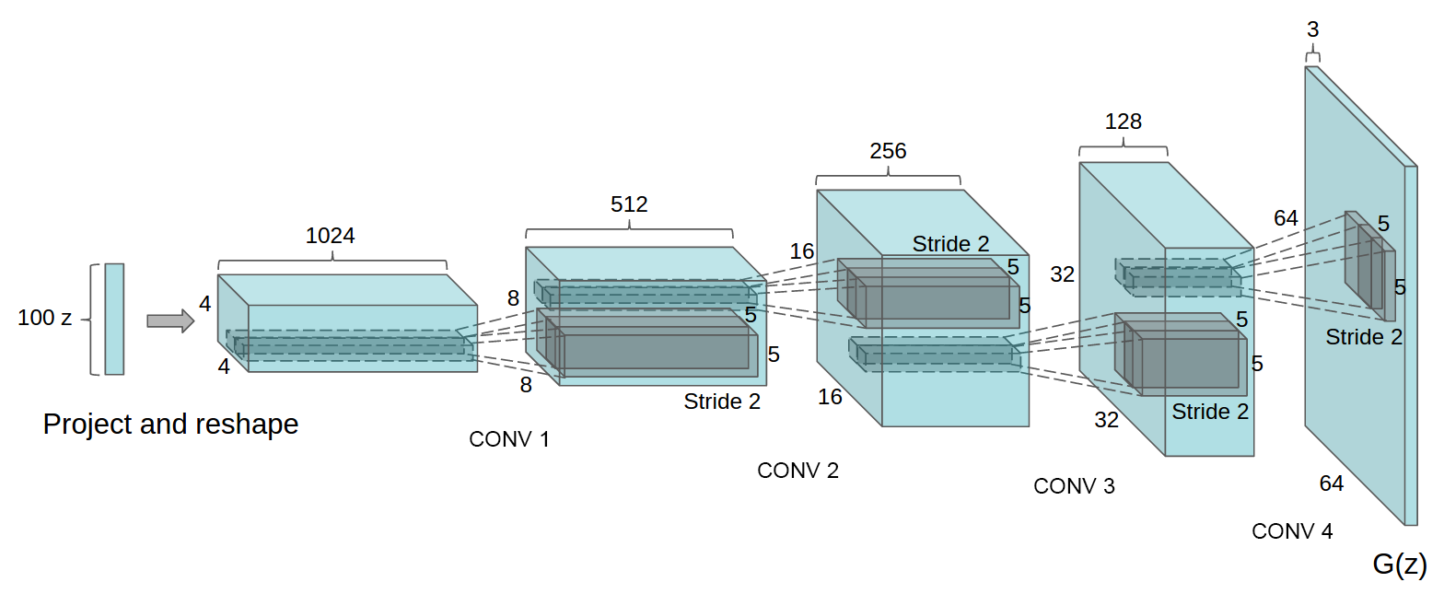
\includegraphics[width=35em]{figures/DCGAN-generator-structure.PNG}
			\caption{DCGAN生成器示意图}
			\label{fig:dcgan-gen-struct}
		\end{figure}
	
		作者在三个数据集上训练了DCGAN,分别是:Large-scale Scene Understanding(LSUN), Imagenet-1k 和一个比较新的面部数据库。
		
		论文中给出了一组训练参数,对调参有一些指导意义:
		
		\begin{enumerate}
			\item 所有模型都使用了batch size=128的梯度下降方法进行训练。
			\item 所有的权值都是用0均值,0.02标准差的正态分布进行初始化
			\item LeakyReLU的斜率值(slope of the leak)都是0.2.
			\item 使用Adam optimizer进行训练。
			\item 作者发现,使用学习率0.001有些高,所以使用了0.0002
			\item Momentum的patient如果是0.9可能会导致训练的波动比较大,所以改成0.5能帮助训练得更稳定一些。
		\end{enumerate}
		
		DCGAN生成器所生成的图片如图\ref{fig:dcgan-res-eph1}和图\ref{fig:dcgan-res-eph5}所示
		\begin{figure}
			\centering
			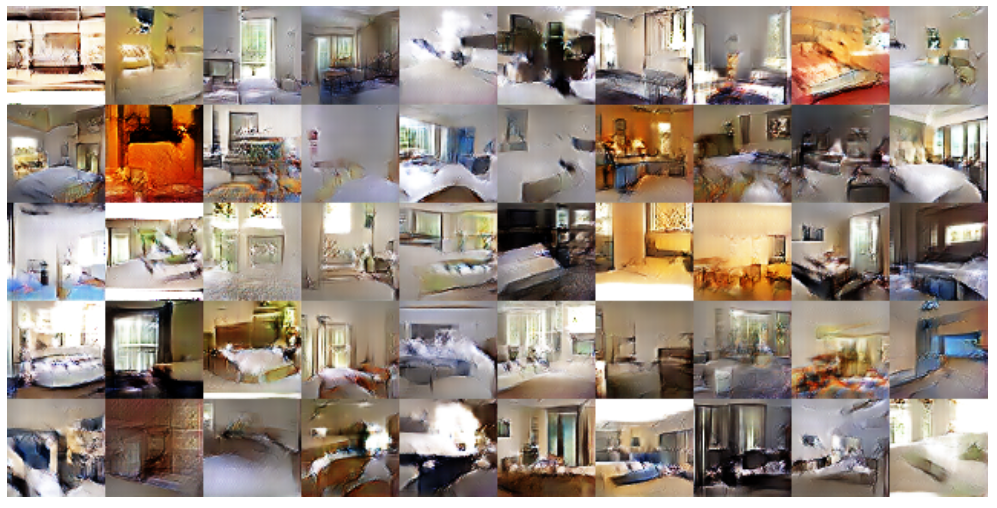
\includegraphics[width=35em]{figures/DCGAN-generated-image-epoch-1.png}
			\caption{当模型训练1个epoch时,生成器产生的结果}
			\label{fig:dcgan-res-eph1}
		\end{figure}
	
		\begin{figure}
			\centering
			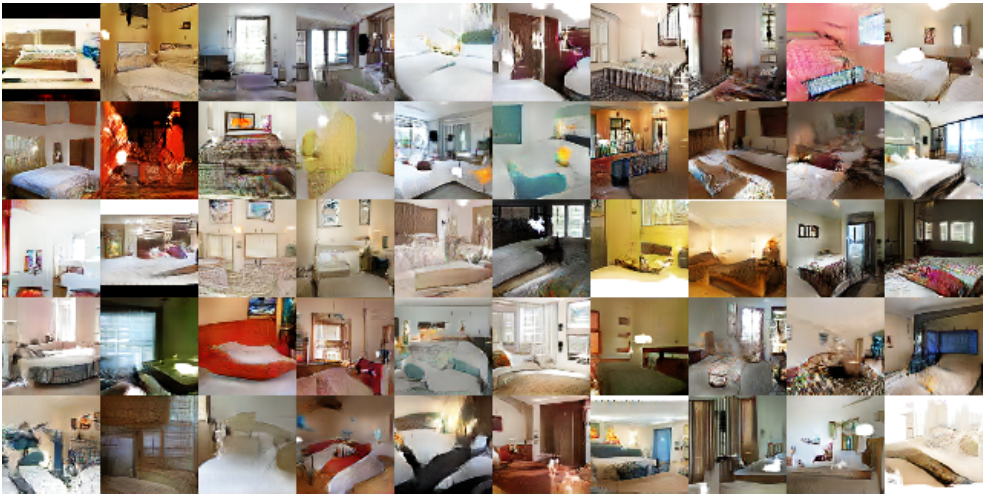
\includegraphics[width=35em]{figures/DCGAN-generated-image-epoch-5.png}
			\caption{当模型训练5个epoch时,生成器产生的结果}
			\label{fig:dcgan-res-eph5}
		\end{figure}
	
		紧接着,作者又用了一些数据来验证DCGAN各方面的能力。
		
		首先,作者使用了DCGAN作为特征抽取器,在CIFAR-10的数据上训练了一个分类器。分类器精度结果如图\ref{fig:dcgan-dis-cifar-fe}
		
		\begin{figure}
			\centering
			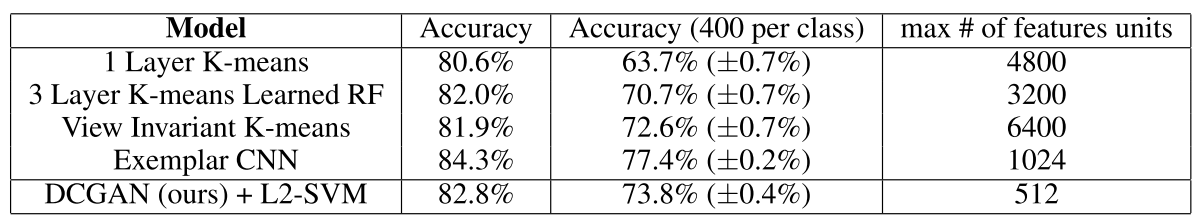
\includegraphics[width=25em]{figures/DCGAN-discriminator-feature-extractor-cifar-10.png}
			\caption{DCGAN的判别器作为CIFAR10特征抽取器的效果}
			\label{fig:dcgan-dis-cifar-fe}
		\end{figure}
	
		这里需要注意的一点是,为了验证DCGAN能够抽取图片的特征,所以作者使用了Imagenet-1k进行训练,然后使用CIFAR-10进行分类性能测试。从表格中能看出,DCGAN+L2-SVM已经能取得不错的效果了。虽然不如Exemplar CNN,但作者觉得后续还有微调的空间。
		
		然后作者又用相似参数进行了街景房间门牌号数据集(StreetView House Numbers dataset, SVHN)做了测试。使用了DCGAN的判别器中抽取到的特征之后,能够达到state-of-the-art的效果(22.48\%错误率)。并且作者证实,达到这个效果并不是因为用了CNN,因为他们发现用了结构完全一样的纯CNN的模型,就达不到这个效果了(28.87\%错误率)。看来对抗学习是有效果的。
		
		性能对比如图\ref{fig:dcgan-dis-svhn-fe}
		
		\begin{figure}
			\centering
			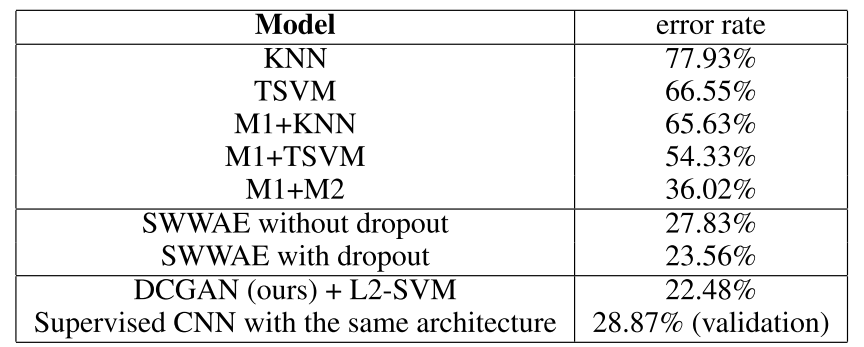
\includegraphics[width=25em]{figures/DCGAN-discriminator-feature-extractor-svhn.png}
			\caption{DCGAN的判别器作为SVHN特征抽取器的效果}
			\label{fig:dcgan-dis-svhn-fe}
		\end{figure}
	
		接下来,作者对网络内部做了可视化。
		
		首先,作者在latent空间进行了简单的修改。作者认为,如果在这个潜在空间做出一些微小的移动导致了语义上的变化(例如多了一张床或者窗户等),这也就说明模型学习到了相关知识的语义上的表达。
		
		图\ref{fig:dcgan-visual-internals-latent}前九行是在9个随机采样的点($z$)处用插值的方法施加微小变化而生成的图片。明显看出这些是在一个卧室中视角做出一些微小的变化。尤其是第六行,这个房间逐渐从一个没有窗户的卧室变成了一间拥有大窗子的卧室。第十行里的电视则慢慢变化为一扇窗子。
		
		\begin{figure}
			\centering
			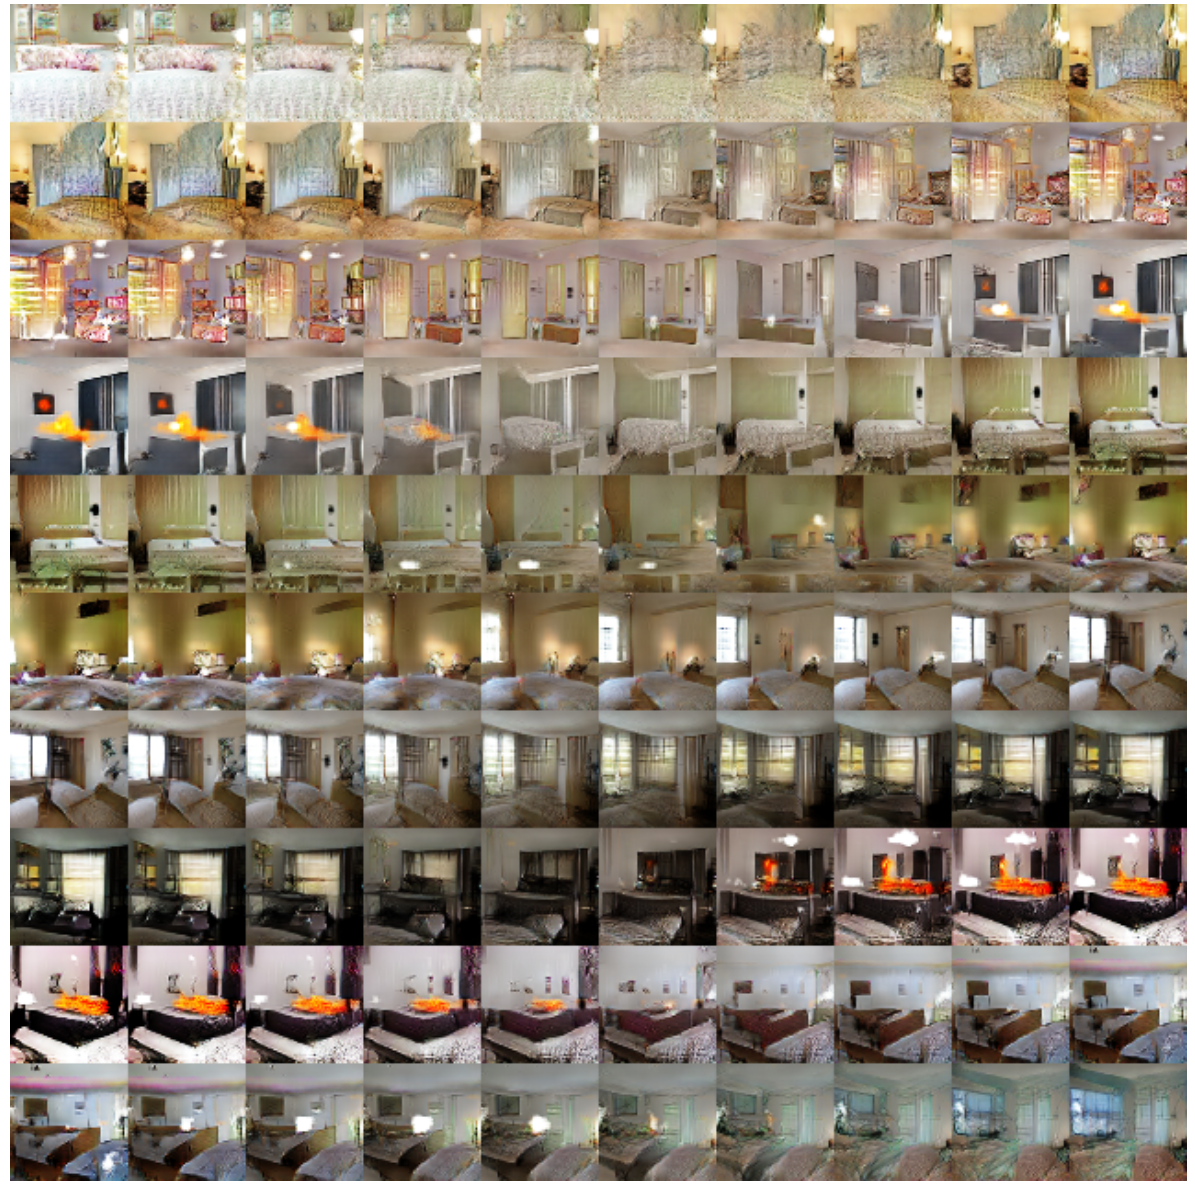
\includegraphics[width=40em]{figures/DCGAN-visualizing-internals-walking-in-latent.png}
			\caption{DCGAN在隐藏域以空间的效果}
			\label{fig:dcgan-visual-internals-latent}
		\end{figure}
		
		然后又做了一个判别器中特征的可视化,如图\ref{fig:dcgan-visual-internals-filters}。
		
		\begin{figure}
			\centering
			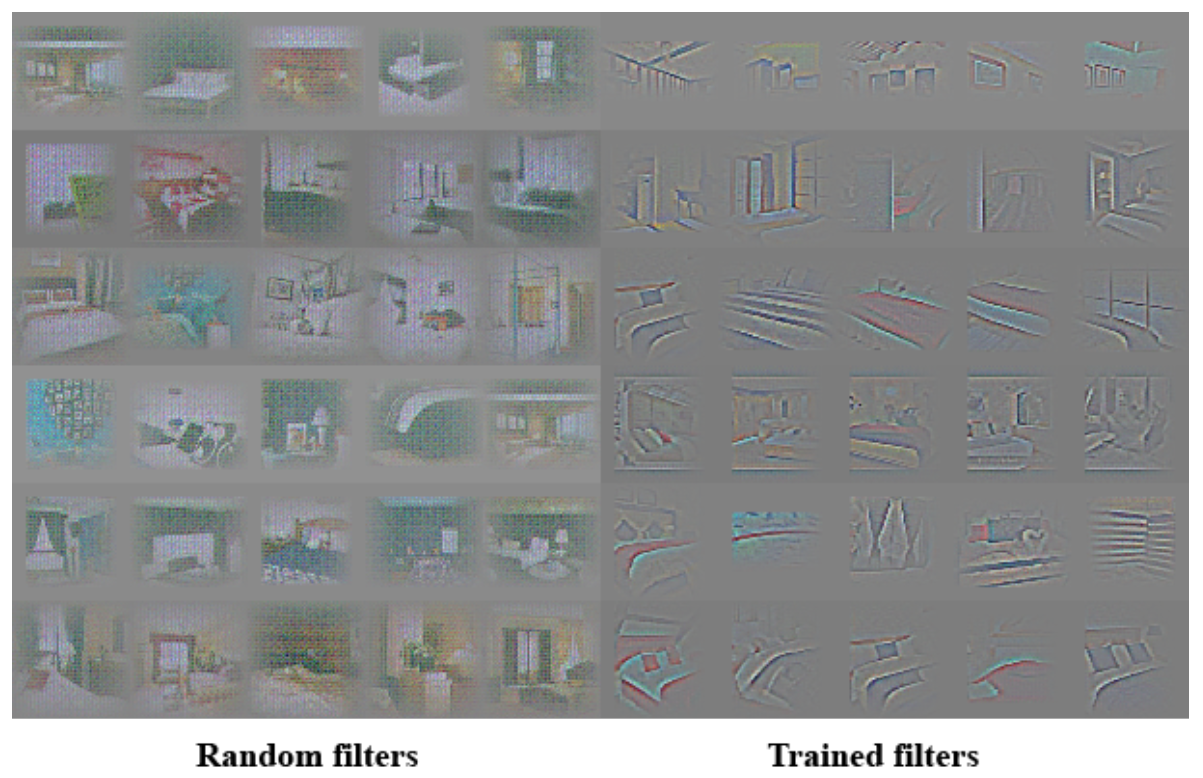
\includegraphics[width=40em]{figures/DCGAN-visualizing-internals-filters.png}
			\caption{DCGAN内部特征的可视化}
			\label{fig:dcgan-visual-internals-filters}
		\end{figure}
		
		在做了这些可视化之后,作者又想尝试操纵生成器的特征表达。
		
		首先,作者尝试去让生成器“遗忘掉”一些特定的对象。如果隐变量中的某些变量决定了对象是否被生成出来,那么删除这些变量,是不是能让生成的图像中不包含这些对象?
		
		原文中关于这个实验记载的不是太明确,下面是我个人的理解:
		
		作者通过一个设计实验来达到这个效果:生成150个样本,其中有52个样本包含了窗子,然后将这个窗子的位置人为地标志出来。然后在倒数第二层卷积层上使用一个logistic regression来判断这个激活函数是否控制着窗子的生成。如果在卷积层的某个filter上发现在标志着窗子的位置范围内有值,则将这个filter抹掉。然后我们会发现,我们生成的图片中的窗子真的被删掉了。
		
		\begin{figure}
			\centering
			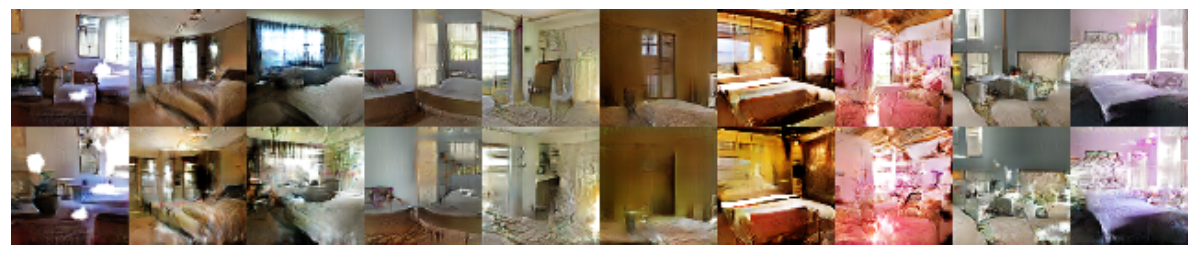
\includegraphics[width=45em]{figures/DCGAN-visualizing-internals-remove-filter.png}
			\caption{删除DCGAN中的部分特征}
			\label{fig:dcgan-visual-internals-remove-filter}
		\end{figure}
	
		在图\ref{fig:dcgan-visual-internals-remove-filter}中,上面一行是带窗子的生成图片,下面一行是抹掉“生成窗子的feature map”之后的生成器所生成的图片。
		
		除了上面这些特性之外,作者还发现了一个有趣的性质,就是图像之间也可以像word embedding一样进行计算的,示意图如图\ref{fig:dcgan-vector-smell}和图\ref{fig:dcgan-vector-glasses}。
		
		\begin{figure}
			\centering
			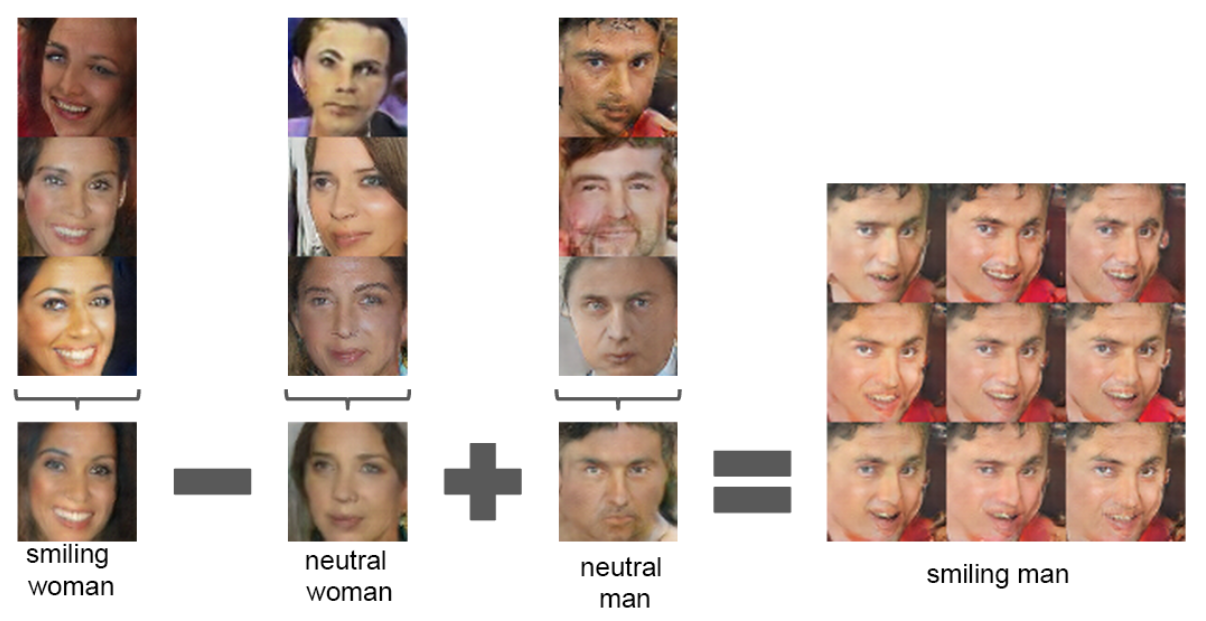
\includegraphics[width=35em]{figures/DCGAN-visualizing-internals-vector-1.png}
			\caption{DCGAN的可加性:smell}
			\label{fig:dcgan-vector-smell}
		\end{figure}
	
		\begin{figure}
			\centering
			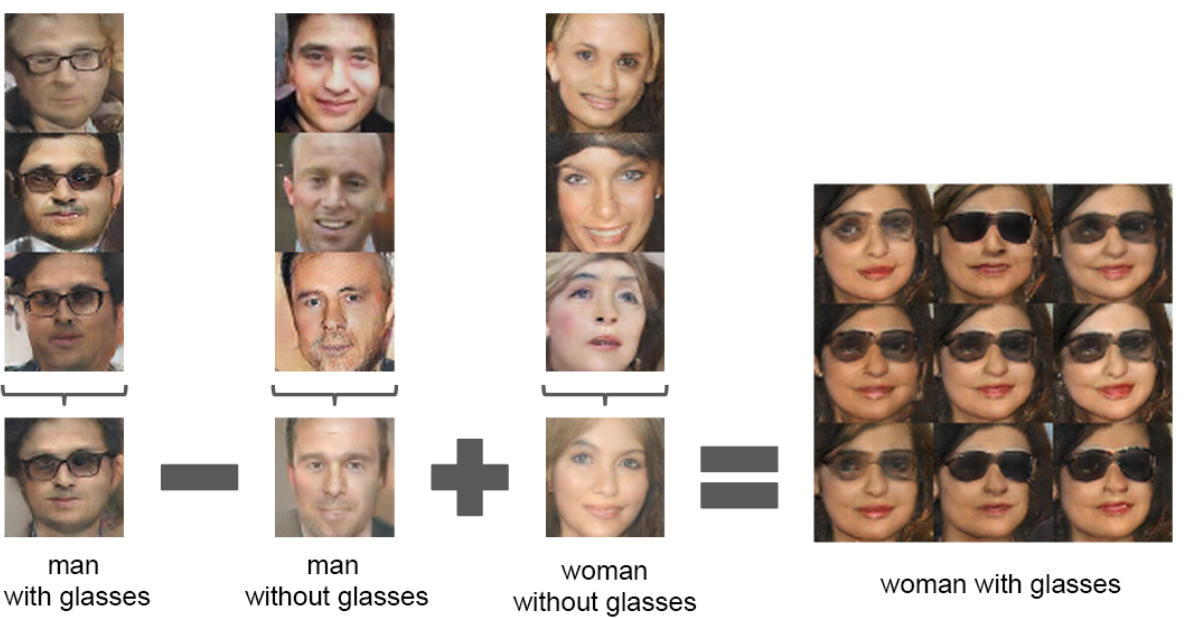
\includegraphics[width=35em]{figures/DCGAN-visualizing-internals-vector-2.PNG}
			\caption{DCGAN的可加性:glasses}
			\label{fig:dcgan-vector-glasses}
		\end{figure}
		
		需要注意的是:首先,用来计算的向量其实是$z$而不是生成图片。其次,应该拿三个类似效果的$z$取平均之后再进行运算。例如我们首先找到能够三个能够产生smiling woman的$z$,取平均之后为$z_1$,然后找到三个能够生成natural woman的$z$取平均后为$z_2$,然后再找到三个能够生成natural man的$z$取平均后为$z_3$,最终经过计算可以得到$z_4=z_1-z_2+z_3$。再用这个得到的$z_4$就能生成smiling man的图片。
		
		类似上面介绍“卧室变换”的方法,作者也有插值的方法做了“面部朝向”的实验。就是说,将脸朝左到朝右的两个$z$,插值出了一大堆“过渡”的$z$,然后得到了如图\ref{fig:dcgan-vector-trans}的效果。
		
		\begin{figure}
			\centering
			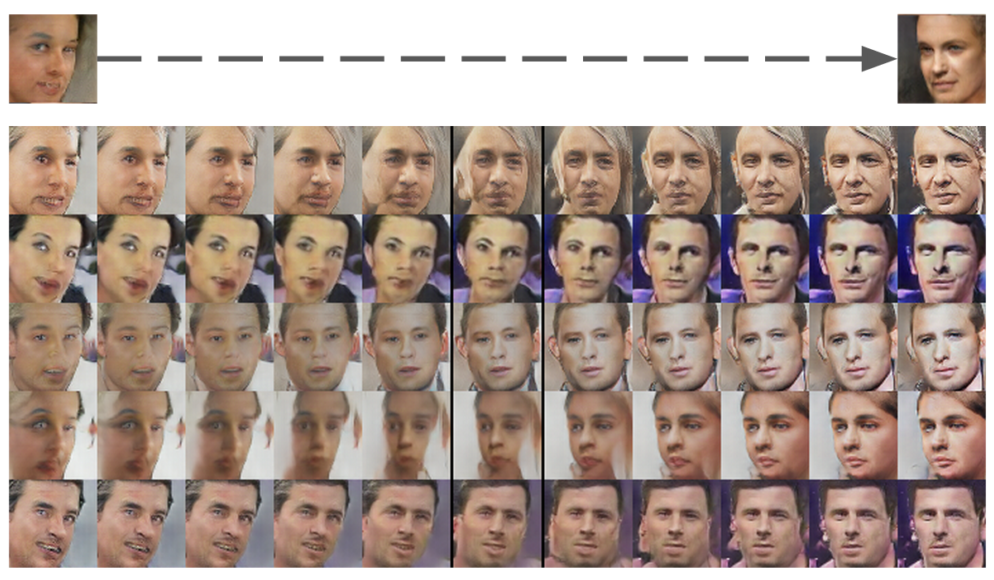
\includegraphics[width=35em]{figures/DCGAN-visualizing-internals-vector-4.png}
			\caption{DCGAN脸部过渡变换}
			\label{fig:dcgan-vector-trans}
		\end{figure}
	
		个人认为这个工作其实挺简单:提出一个模型和训练方案,以解决GAN不稳定的问题。但这篇文章的价值其实体现在了两个方面:1,作者深厚的调参功底和实验技巧并在文章中总结出了大量的经验,对使用GAN的后来者有明显的借鉴作用。2,作者做了大量的实验,并且尽可能地去\emph{分析}GAN在“Representation Learning”中的奇效。所以这篇文章的工作还是相当充分的!
		
	\end{section}

	\begin{section}{Laplacian Generative Adversarial Networks}
		
		在GAN的日常应用中我们会发现,用GAN生成的图片其实并不是很逼真。尤其是在高分辨率的情况下,图片看起来明显不自然。
		
		所以在研究了用GAN生成图片的框架之后,很多研究者就开始研究如何让GAN生成的图片看起来更加地自然。一个比较有效果的工作就是Emily Denton et al.的这篇文章\cite{denton2015deep}。
		
		这篇文章使用级联的方式将很多个由卷积模型组成的生成式网络组合在一起。如同人类作画一样,逐步添加细节,一步一步让内容更加真实,实现了一个“逐步求精”(coarse-to-fine)的过程。这个组合框架被称为Laplacian pyramid,所以这个这篇论文的题目就叫做Deep Generative Image Models using a Laplacin Pyramid of Adversarial Networks。下面简称这个模型为LAPGAN。
		
		回顾一下GAN:由生成器和判别器组成;生成器输入一串噪声,输出尽可能逼真的图片;判别器输入一张图片,尽可能正确地判断这张图片是由生成器产生的,还是一张真正的图片。这个模型的训练目标是这个:
		
		\begin{equation}
			\mathop{\min}_{G}\mathop{\max}_{D}V(D,G)=\mathbb{E}_{\boldsymbol{h}\sim p_{\text{Data}}(\mathbf{h})}\left[\log D(\boldsymbol{h})\right]+\mathbb{E}_{\boldsymbol{z}\sim p_{\text{Noise}}(\mathbf{z})}\left[\log(1-D(G(\boldsymbol{z})))\right].
		\end{equation}
		
		而LAPGAN并不是用这个最基本的GAN模型,而是用第二节中提到的CGAN(Conditional GAN)。在CGAN中,增加了一个叫做Condition的向量,作为对“控制信息”的编码。这个控制信息可能是图像、标签的one-hot表示、文本等任何内容。这时候,训练目标就变成了这个:
		
		\begin{equation}
			\mathop{\min}_{G}\mathop{\max}_{D}V(D,G)=\mathbb{E}_{\boldsymbol{h},\boldsymbol{l}\sim p_{\text{Data}}(\mathbf{h},\mathbf{l})}\left[\log D(\boldsymbol{h},\boldsymbol{l})\right]+\mathbb{E}_{\boldsymbol{z}\sim p_{\text{Noise}}(\boldsymbol{z}),l\sim p_{l}(\mathbf{l})}\left[\log(1-D(G(\boldsymbol{z},\boldsymbol{l}),\boldsymbol{l}))\right].
		\end{equation}
		
		这里面这个$l$就是控制变量,例如在MNIST数据集上生成手写数字,这个$l$就可以是一个表示类别的10维的one-hot向量。
		
		LAP(Laplacian Pyramid)的主要思想就是考虑计算“将小图像上采样得到的图像”与“图像本身”的残差。下面是一些形式化的定义。
		
		首先我们定义两个函数。$d(.)$为降采样:例如有一张$j\times j$大小的图像$I$,则$d(I)$的尺寸就是$j/2\times j/2$。另一个函数是$u(.)$为上采样,$u(I)$的尺寸是$2j\times 2j$。
		
		然后,可以定义一个Gaussian Pyramid $\mathcal{G}(I)=\left[I\_0,I\_1,\dots,I\_K\right]$。其中$I\_0=I$,$I\_k$就是将降采样连续用了$k$次。例如$I\_1=d(I)$、$I\_2=d(d(I))$以此类推。
		
		Laplacian Pyramid则是由一组系数$h\_k$组成。表达式是:
		
		\begin{equation}
			h_k=\mathcal{L}_k(I)=\mathcal{G}_k(I)-u(\mathcal{G}_{k+1}(I))=I_k-u(I_{k+1})
		\end{equation}
		
		有了这一组参数,想要重构图像,就可以这样:$I\_k=u(I\_{k+1})+h\_k$。重构图片的时候从这个公式的第$K$项开始,逐步向前进行,最终图像$I=I\_0$。
		
		LAPGAN就是利用了这个思想。通过模型,训练出一个能产生这个系数的生成器,使用“对小图像上采样再叠加这个系数”的方式,从而使低分辨率图像逐步变清晰。
		
		也就是说,整个框架“画”出来的图像,是通过一组GAN,利用这样的方式画出来:
		
		\begin{equation}
			\tilde{I}_k=u(\tilde{I}_{k+1})+\tilde{h}_k=u(\tilde{I}_{k+1})+G_k(z_k,u(\tilde{I}_{k+1}))
		\end{equation}
		
		从公式中可以发现,$\tilde{h}\_k$实际上是由$G\_k$通过$z\_k$和$u(\tilde{I}\_{k+1})$产生的。其中$z\_k$就是GAN中的输入噪声,$u({\tilde{I}\_{k+1}})$就是CGAN中的控制条件。
		
		生成流程如图\ref{fig:lapgan-gene-structure}所示。
		
		\begin{figure}
			\centering
			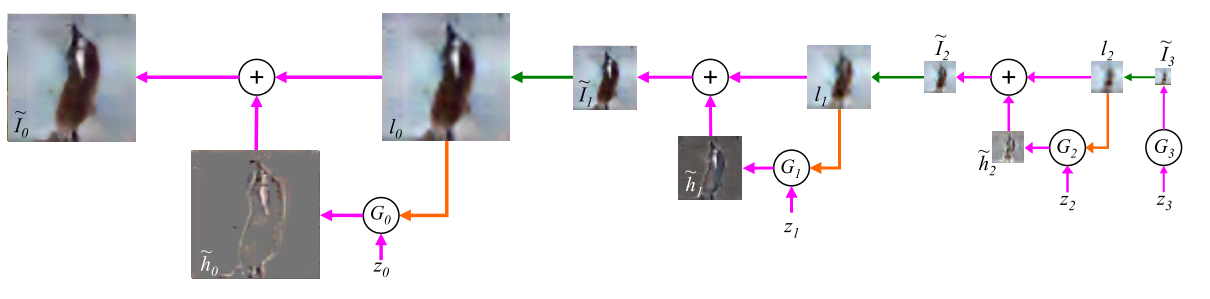
\includegraphics[width=40em]{figures/LAPGAN-generator-structure.png}
			\caption{LAPGAN生成器的基本结构}
			\label{fig:lapgan-gene-structure}
		\end{figure}
	
		开始训练时,我们先用最后一级的生成模型$G\_K$输入噪声$z\_k$产生一个$\tilde{I}\_3$。为了统一模型的架构,此时我们可以设置让$\tilde{I}\_{K=1}=0$,也就是说这个GAN中并没有控制变量的输入。之后就可以按照上面的公式一层一层将这个模型串起来,最终得到一个更高分辨率的图像。
		
		现在问题来了,我们应该如何训练这个生成器G呢?训练生成器,就需要对抗学习的方法。我们可以将这个模型转换成为这个架构(只在训练时使用的架构),如图\ref{fig:lapgan-structure}。
		
		\begin{figure}
			\centering
			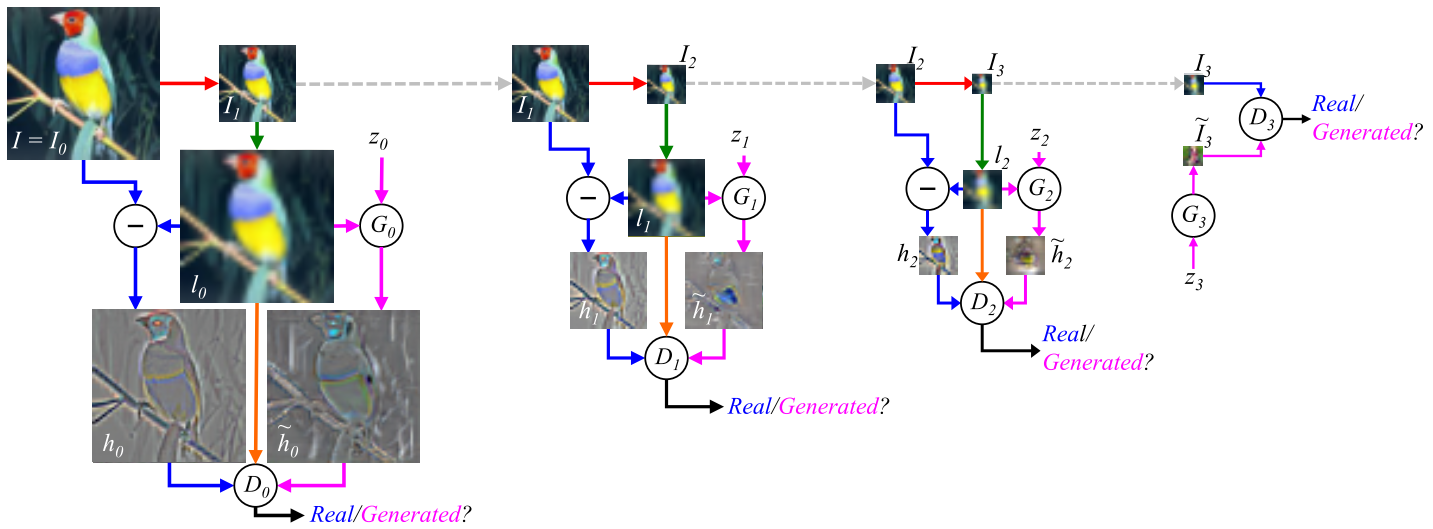
\includegraphics[width=40em]{figures/LAPGAN-general-structure.png}
			\caption{LAPGAN的基本架构}
			\label{fig:lapgan-structure}
		\end{figure}
	
		在这个架构下,我们用来训练的顺序跟生成图片的顺序刚好相反,即从原图开始,逐渐向金字塔顶端进行训练。以上图中的第一张图片为例,原图$I\_0=I$,首先对原图进行降采样得到$I\_1$,然后再对$I\_1$上采样得到$l\_0$。这时候,我们将原图$I\_0$与降采样后上采样得到的模糊图$l\_0$做差,计算出来的残差就是$h\_0$。在训练中,我们认为这个$h\_0$就是GAN中可以被判别器标记为真实(Real)的样本。另一方面,我们的CGAN模型,通过输入一段噪声$z\_0$和降采样后上采样的模糊图片$l\_0$,就能生成一个$\tilde{h}\_0$。而判别器的功能,就是来判断输入的内容究竟是真实的?还是生成的?在这样的架构之下,系统就能够学习到“将低质量图像变成高质量图像的画笔”。在按照前面一张图片所介绍的过程,就可以生成高质量的图片了!
		
		实验结果就不展开讨论了,具体效果如图\ref{fig:lapgan-result}。
		
		\begin{figure}
			\centering
			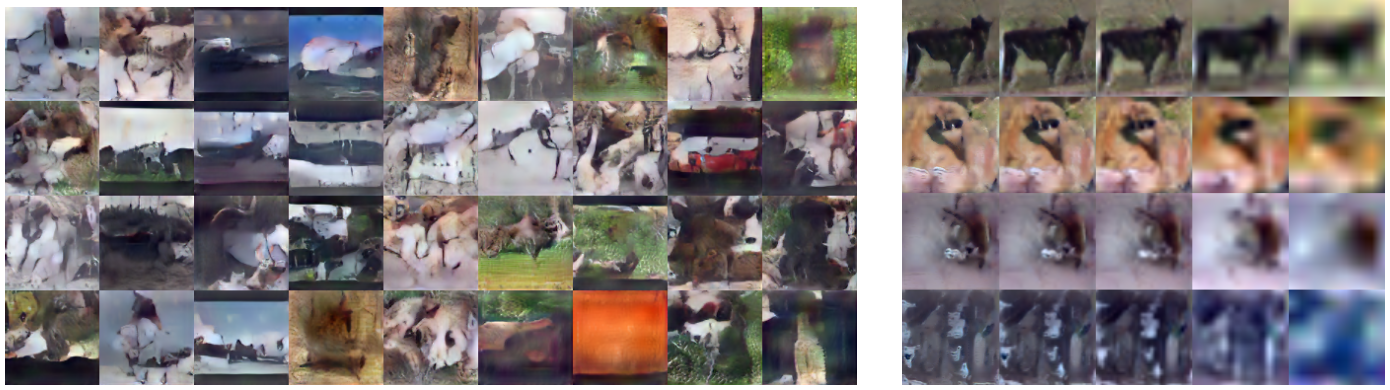
\includegraphics[width=45em]{figures/LAPGAN-experiment.png}
			\caption{LAPGAN生成结果示意图}
			\label{fig:lapgan-result}
		\end{figure}
	
		从这个结果中我们能够理解到Laplacian Pyramid的核心思想。如果我们将一张图降采样再上采样,得到的图片势必会变模糊,如果我们能得到模糊图片和原始图片的插值,也就意味着我们可以将一张分辨率不高的图片,通过叠加这个残差来提升其分辨率。
		
		这种方法并不是学习“如何将分辨率低的图片变成分辨率高的图片”,而是学习能够让分辨率低的图片变成分辨率高的图片的“画法”。这个思想感觉在很对场景都会有应用。即学习到从A到B的映射或许很难,但我们可以捕捉到A和B之间差值的规律,通过对A增加这个差值而得到B,这可能会把问题的规模变得更简单。
		
		这篇文章的另一个启示就是,不要拘泥于GAN中判别器用来判断“真假”的这个固有思维。其实,判别器就是一个二类分类器,它可以用作区分图片是真实的还是生成的,也可以区分输入是“我们所定义的”合理的、还是不合理的。
		
	\end{section}


	\begin{section}{Generative Adversarial Text to Image Synthesis}
		前面几节介绍了几个GAN的变种,但是那些文章始终围绕着“生成高质量图像”这个topic。如何让模型按照我们“复杂的需求”生成图像呢?这就是这篇文章\cite{reed2016generative}想要解决的问题。
		
		这篇文章介绍了一种能够将人工编写一句描述性文本直接转换成为图像。如图\ref{fig:image-synthesis-exp}。
		
		\begin{figure}
			\centering
			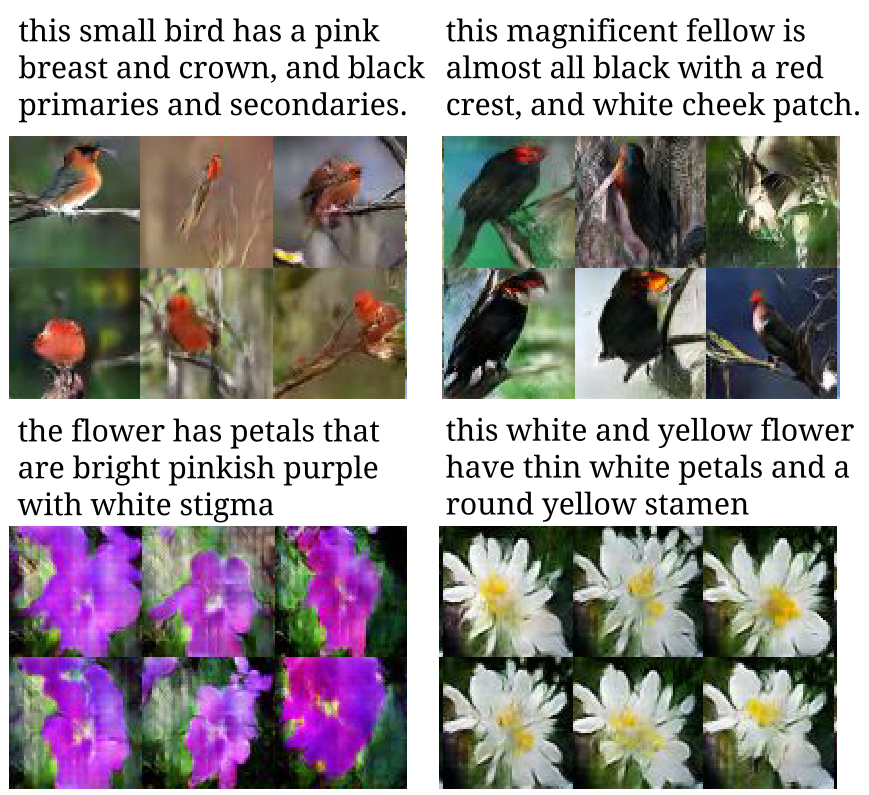
\includegraphics[width=20em]{figures/image-synthesis-prelude-demo.png}
			\caption{由描述性文本生成图片}
			\label{fig:image-synthesis-exp}
		\end{figure}
	
		这是一个看起来很fancy的工作,因为它适用范围相当广,但这个问题显然还是挺困难的,所以还没有得到非常良好的解决。
		
		这项工作主要面临两大挑战:
		
		\begin{enumerate}
			\item 学习到能够捕捉到重要的视觉细节的文本特征表达 (learn a ext feature representation that captures the important visual details)
			\item 使用这些特征来合成一些让人们误以为真的图片 (use these features to synthesize a compelling image that a human might mistake for real).
		\end{enumerate}
		
		这两项挑战虽然具有难度,但幸运的是,由于近年来深度学习的兴起,这两项挑战的子问题“自然语言表达”和“图像合成”已经得到了一定程度的解决。
		
		但是,仍然存在着一个没能很好解决的问题:按描述生成图片(即以文本描述为条件的图像概率分布)是一个非常多模态的问题,也就是说,很有可能会有很多图片都能套用到相同的解释之上。
		
		如果将图像生成反过来、即进行“图像到文本”的caption工作,这个情况依然是个麻烦。然而由于可以使用链式法则将一个序列化的问题解构并最终让这个task可解。例如可以训练一个模型,给定这张图片和之前所有的token来预测下一个token是什么,换句话说,这个模型其实就是一个well-defined的预测问题。
		
		作者认为可以用GAN很自然地来解决这个conditional multi-modality问题。这篇文章的主要贡献就是实现了一个简单高效的GAN架构和训练策略,使得从人工编写的描述文本合成鸟与花的图片成为可能。
		
		文章中用到的主要是在第三节中曾经介绍过的DCGAN模型。本文中的应用是以hybird character-level convolutional RNN encode的text feature作为输入条件。生成器$G$和判别器$D$在前向inference的时候都以这个text feature作为条件。
		
		网络的整个结构如图\ref{fig:image-synthesis-struct}所示。
		
		\begin{figure}
			\centering
			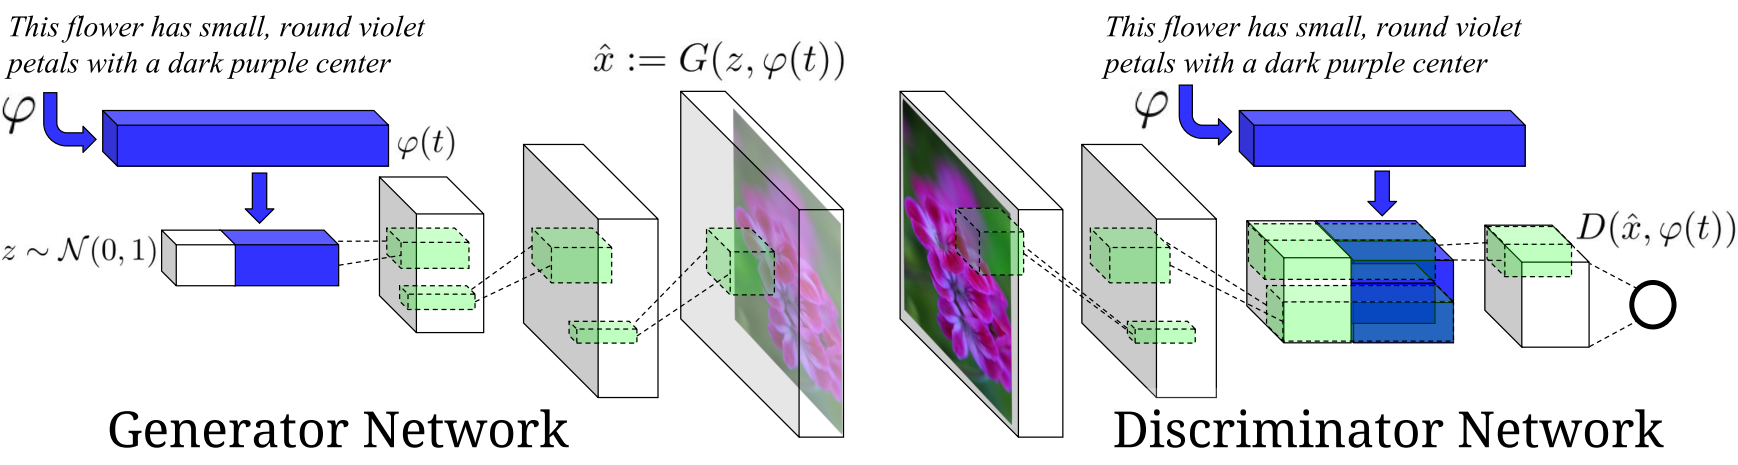
\includegraphics[width=35em]{figures/image-synthesis-structure.png}
			\caption{图片生成的整体结构}
			\label{fig:image-synthesis-struct}
		\end{figure}
		
		网络如同其他GAN一样,分为生成器$G$和判别器$D$两个部分。由于是条件GAN,所以生成器的输入不止有随机采样的噪声$z\sim \mathcal{N}(0,1)$,更有一个text feature(即途中蓝色部分)。这个text feature是由text encoder $\phi$ 生成的,如果text query为 $t$ 则这个text feature就是 $\phi(t)$。
		
		通常需要将描述文本使用一个全连接层压缩到一个较小维度之后(一般是128维),并使用leaky ReLU再与噪声向量$z$拼接在一起,作为生成器的整体的输入。
		
		紧接着,后续的前向推断过程就是一个解卷积网络:即一张合成的图片$\hat{x}$通过$\hat{x}\leftarrow G(z,\phi(t))$被生成出来。
		
		再来看判别器D。前面几层使用了stride-2卷积层并使用了spatial batch normalization和leaky ReLU。并且仍然像以前一样使用一个全连接层接上一个rectifier来减少描述文本embedding $\phi(t)$的维度。当判别器的维度是$4\times 4$时,将这个描述文本的embedding复制多份,并在深度上与图片进行拼接。然后在拼接之后的新tensor上继续执行一个卷积操作,然后再计算得分。这便是整个框架在inference的流程。
		
		说完了inference,就该说说train了。该如何去train这个模型?训练条件GAN的最直接的方法就是将图片和description embedding看作是联合的样本,通过观察判别器判断“生成的图片+文本”这个整体是真的还是假的。不过这个方法有些naive:并没有在训练中给判别器提供“是否按照描述正确生成了图像”的信息。
		
		但事实上,这种CGAN的训练过程会与非CGAN训练过程有些不同。在训练的初期,由于生成的图片大多不靠谱,所以判别器将会拒绝大部分生成的图片,这也就相当于无视了condition的存在。然而一旦生成器学习到了如何产生靠谱的图片,生成器也一定会学习到如何生成“符合条件”的图片。然后判别器也会去学习去判断生成的内容是否符合条件限制。
		
		在这naive GAN的情况下,判别其将会观察到两种不同的输入:正确的图片并且配上了正确的文本,以及错误的图片配上了随意的文本。所以,需要分开记录这两种不同的错误来源:不真实的图片(配上任何文本),以及真实图片但条件信息匹配错误。
		
		作者修改了GAN的训练算法来将这两种不同的错误分开。除了real/fake这两种输入以外,作者又增加了第三种输入“真实的图片配上错误的文本”,而判别器也必须要能把这种错误给区分出来。
		
		整个训练算法:
		
		\begin{algorithm}[H]
			\algsetup{linenosize=\tiny}
			\caption*{\textbf{Algorithm} GAN-CLS training algorithm with step size $\alpha$, using minibatch SGD for simplicity.}
			\begin{algorithmic}
				\REQUIRE minibatch images $x$, matching text $t$, mismatching $\hat{t}$, number of training batch steps $S$
				\FOR{$n=1,\dots,S$}
				\STATE $h\leftarrow\phi(t)$ //encode matching text description
				\STATE $\hat{h}\leftarrow\phi(\hat{t})$ //encode mis-matching text description
				\STATE $z\sim\mathcal{N}(0,1)^Z$ //draw sample of random noise
				\STATE $\hat{x}\leftarrow G(z,h)$ //forward through generator
				\STATE $s_r\leftarrow D(x,h)$ // real image, right text
				\STATE $s_w\leftarrow D(x,\hat{h})$ // real image, wrong text
				\STATE $s_f\leftarrow D(\hat{x},h)$ // fake image, right text
				\STATE $\mathcal{L}_D\leftarrow\log(s_r)+(\log(1-s_w)+log(1-s_f))/2$  
				\STATE $D\leftarrow D-\alpha\partial\mathcal{L}_D/\partial D$ // update discriminator
				\STATE $\mathcal{L}_G\leftarrow\log(s_f)$
				\STATE $G\leftarrow G-\alpha\partial\mathcal{L}_G/\partial G$ // update generator
				\ENDFOR
			\end{algorithmic}
		\end{algorithm}
		
		这个伪代码其实也是通俗易懂:
		首先,将正确的和错误的文本信息encode成$h$和$\hat{h}$,然后采样出一个随机噪声,然后用正确的encode和随机噪声,产生一组fake图片。然后分别计算三个不同的判别其判别的结果:真实图片正确文本、真实图片错误文本、生成图片正确文本。然后再通过后面的公式计算判别器的损失函数,进而更新判别器。然后再计算生成器的损失函数,并更新生成器。最终完成整个流程。
		
		上面介绍的GAN-CLS方法是训练这个模型的方法之一,文中作者提出了另一种训练方法。
		
		深度学习的目的在于学习一个良好的特征表达。一些文章证明,在embedding pairs之间的插值如果在数据流形附近,就说明这个特征选得好。所以我们可以创建大量的额外的text
		embedding,这些text embedding其实是通过训练集标注的text
		embedding通过插值得到的。换句话说,这些插值得到的embedding是无法直接对应到人工文本标注上的,所以这一部分数据时不需要标注的。想要利用这些数据,只需要在生成器的目标函数上增加这样一项:
		
		\begin{equation}
			\mathbb{E}_{t_1,t_2\sim p_{\text{data}}}\left[\log(1-D(G(z,\beta t_1+(1-\beta)t_2)))\right]
		\end{equation}
		
		这个公式相当于综合考虑了两个text embedding $t\_1$和$t\_2$的插值点。通常在实际应用中使用$\beta=0.5$效果就不错了。
		
		最后是实验部分,效果如图\ref{fig:image-synthesis-result}。
		\begin{figure}
			\centering
			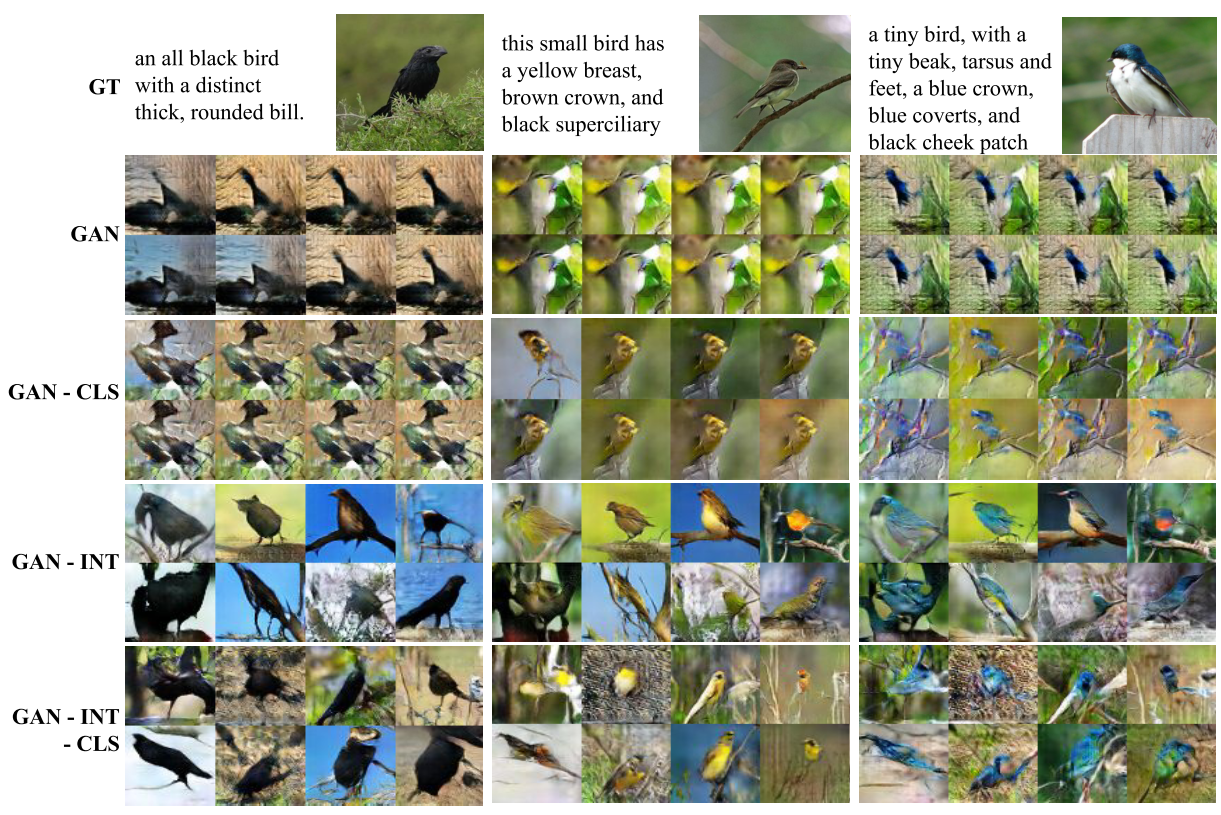
\includegraphics[width=35em]{figures/image-synthesis-experiment.png}
			\caption{由描述性文本生成图片}
			\label{fig:image-synthesis-result}
		\end{figure}
	\end{section}

\bibliographystyle{plain}
\bibliography{document.bib} 

\end{document}